\documentclass[11pt]{article}
\usepackage[margin=1in]{geometry}
\usepackage{amsmath,amssymb,booktabs,graphicx,setspace,caption,hyperref}
\usepackage[T1]{fontenc}
\usepackage{mathpazo}
\setlength{\parindent}{0pt}
\setlength{\parskip}{0.6em}
\captionsetup{font=small,skip=6pt}
\title{Panel MS-AR(1): common intercept and linear trend\\[0.4em]\large Full sample, seasonally adjusted real GDP per worker}
\author{}
\date{}
\begin{document}
\maketitle
\section{Model}
All countries and all years in the 2026-09-17 panel. No country random effects and no catch-up term.
\begin{align}
y_{it} &= a + g\, t + z_{it}, \\
z_{i,t+1} &= \bigl(1-\rho(s_{it})\bigr)\mu(s_{it}) + \rho(s_{it})\, z_{it} + \sigma(s_{it})\,\varepsilon_{it}, \\
s_{i,t+1} &\sim \Pi(\,\cdot\mid s_{it}).
\end{align}
Three regimes. The unconditional mean of the cycle is restricted to $E[z]=0$ (the median regime mean is not pinned at 0). $\sigma$ and $\rho$ switch, with $|\rho|<0.99$. Standard errors are delta-method from a numerical Hessian.
\clearpage
\section{Common intercept and linear trend, full sample}
2026-09-17 SA panel, full sample, $y_{it}=a+gt+z_{it}$, $E[z]=0$. 74 countries, 8670 observations, 1950-Q1--2026-Q2. Fitted countries: 74. Observations: 8670. Log-likelihood: 22608.76.
Common intercept $a=-5.2386$ (0.0684). Common slope $g=0.0079$ (0.0005).
\begin{table}[h]
\centering
\caption{Regime AR(1), transition matrix, and ergodic $\pi$. Columns are regimes.}
\begin{tabular}{lccc}
\toprule
 & (0) & (1) & (2) \\
\midrule
$\mu$ & -0.9769 & -0.7825 & 0.9710 \\
 & (0.0864) & --- & (0.0581) \\ \addlinespace
$\sigma$ & 0.0695 & 0.0161 & 0.0091 \\
 & (0.0019) & (0.0004) & (0.0001) \\ \addlinespace
$\rho$ & 0.9900 & 0.9900 & 0.9900 \\
 & (0.0000) & (0.0000) & (0.0000) \\ \addlinespace
$\Pi_{0\cdot}$ & 0.7509 & 0.1688 & 0.0803 \\
 & (0.0229) & (0.0204) & (0.0114) \\ \addlinespace
$\Pi_{1\cdot}$ & 0.0593 & 0.9360 & 0.0048 \\
 & (0.0062) & (0.0063) & (0.0020) \\ \addlinespace
$\Pi_{2\cdot}$ & 0.0280 & 0.0013 & 0.9707 \\
 & (0.0035) & (0.0017) & (0.0033) \\ \addlinespace
$\pi$ & 0.1453 & 0.3924 & 0.4624 \\
 & (0.0118) & (0.0302) & (0.0321) \\ \addlinespace
\bottomrule
\end{tabular}
\end{table}
\begin{figure}[h]
\centering
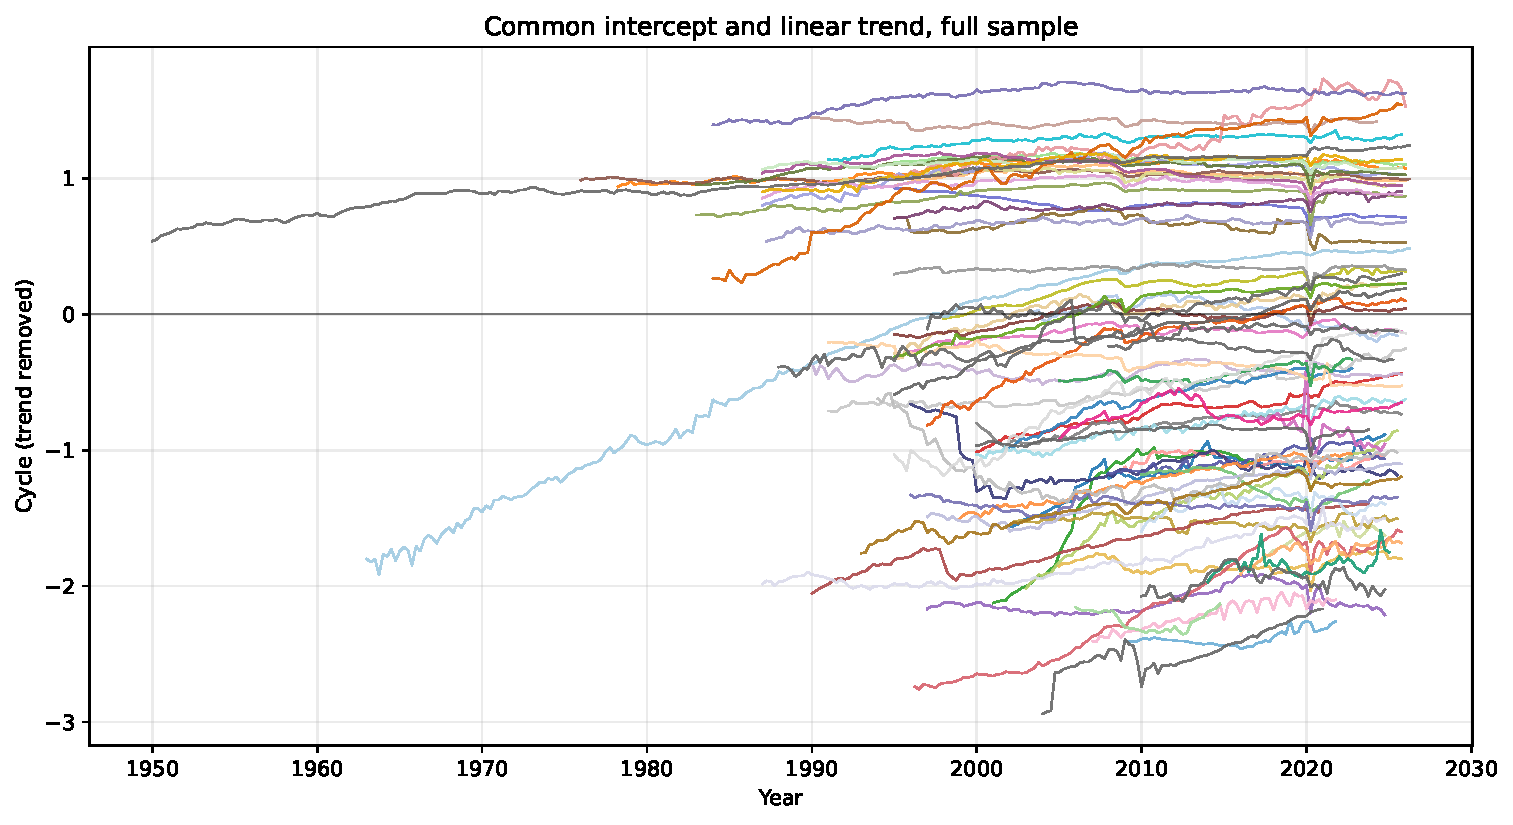
\includegraphics[width=0.75\textwidth]{figs/cycle_common_full.pdf}
\caption{Country cycles after removing the common intercept and the linear trend.}
\end{figure}
\end{document}
